\section{Theory}
\label{sec:Theory}
\subsection{The Sagnac Interferometer}
\label{sec:The_Sagnac_Interferometer}
A Sagnac interferometer is a device built out of multiple mirrors and a polarising beam splitter cube (PBSC). Its purpose is to split a laser beam entering the interferometer into two beams, which can then be redirected over different path. A sketch of the device can be seen in \autoref{fig:interferometer}.\\
To split the beam, it first goes through the PBSC at a $45$ degree angle to the beam. This reflects s-polarised light, while transmitting p-polarised light. The beams then get reflected thrice via multiple mirrors to reenter the PBSC. A portion of each of these beams is then transmitted/reflected into the output area, as shown in \autoref{fig:interferometer}.\\
\begin{figure}
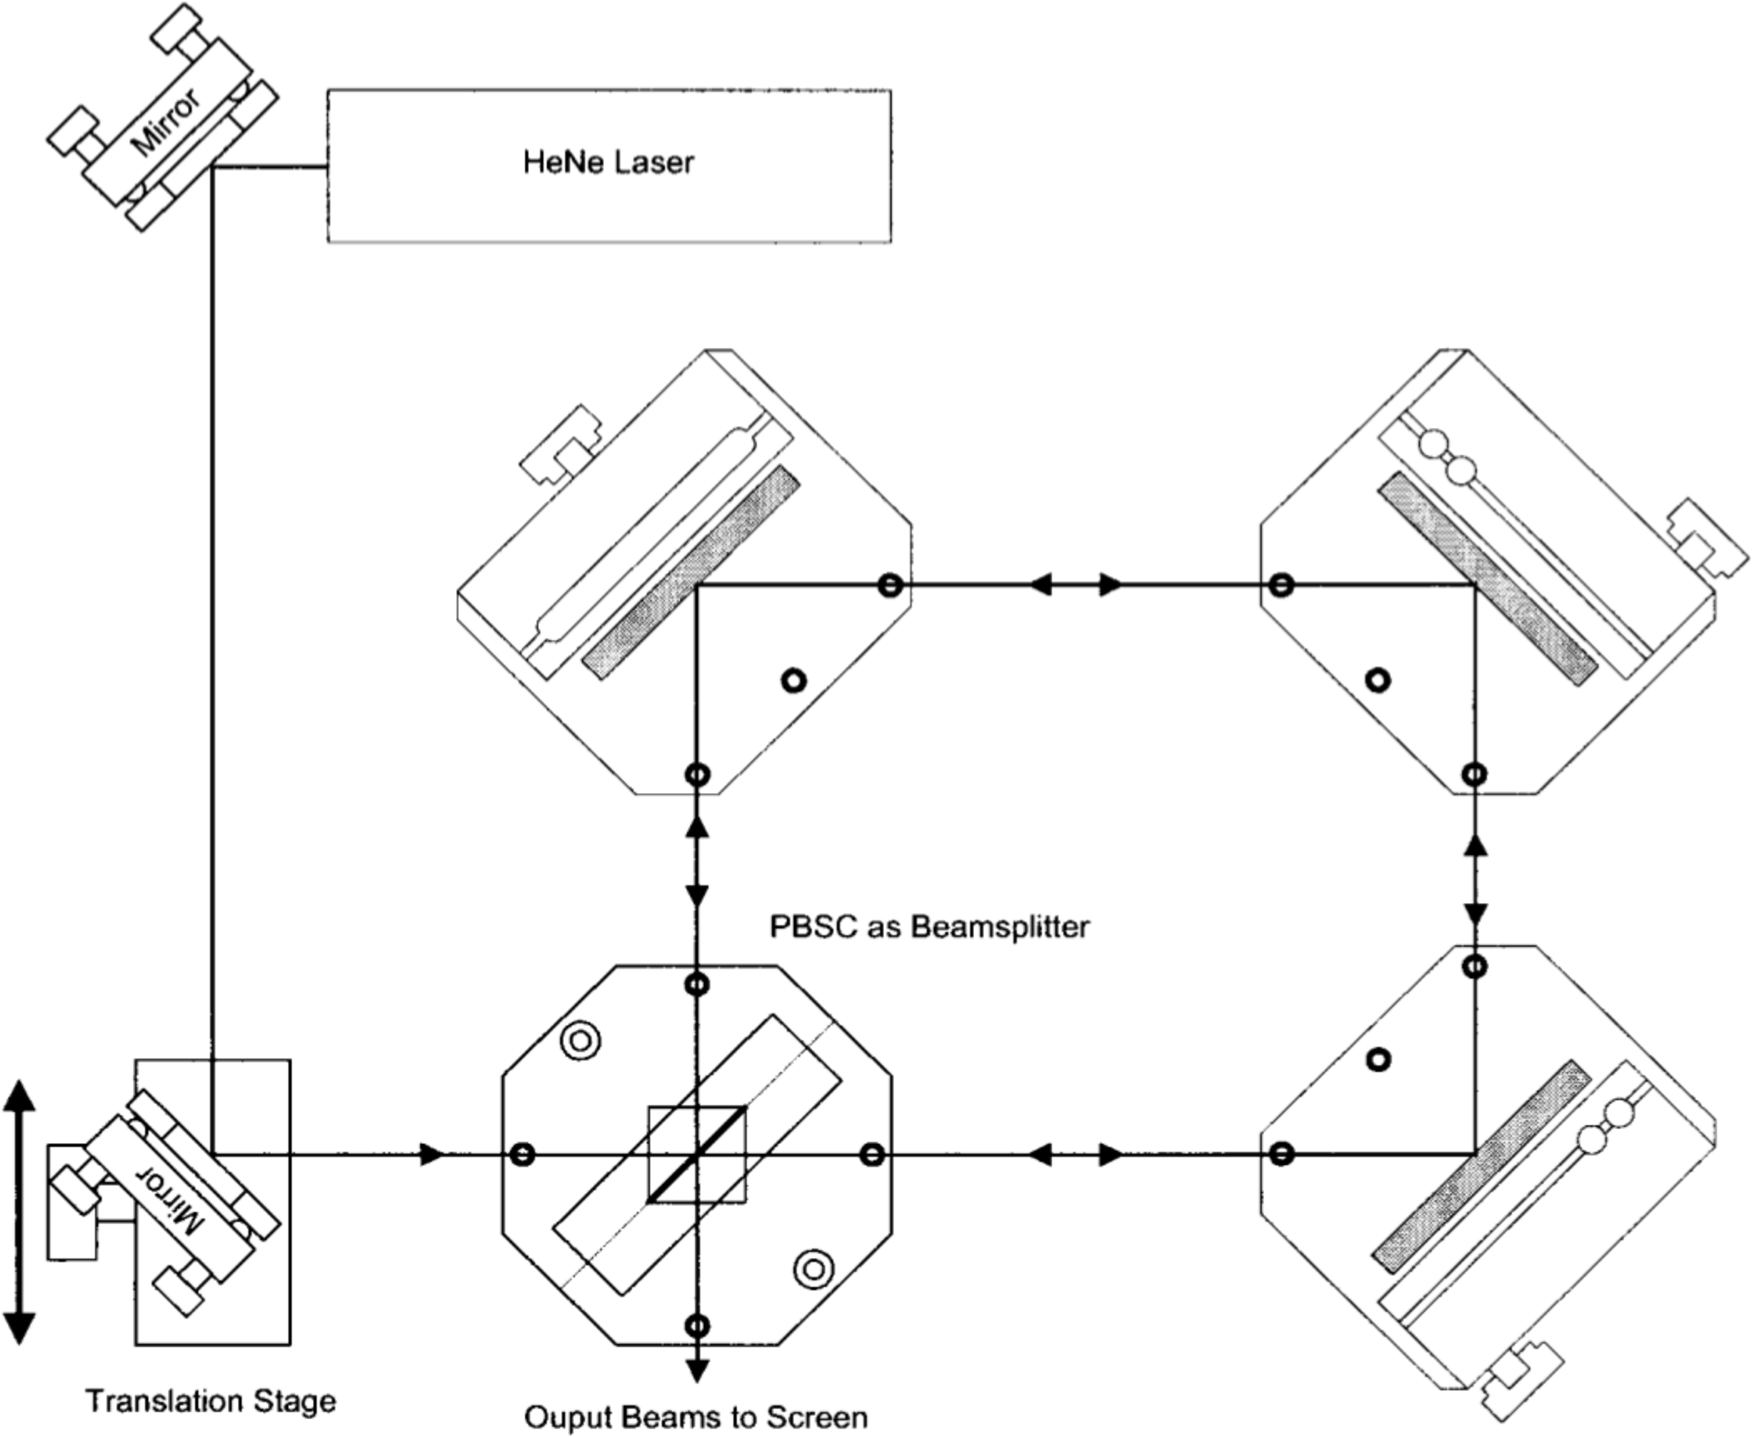
\includegraphics[width=\linewidth]{./figures/aufbau.pdf}
\caption{The Sagnac Interferometer}
\label{fig:interferometer}
\end{figure}
If the interferometer is perfectly adjusted, the resulting beams will overlap at all stages of the interferometer. To manipulate each beam individually, it is necessary to separate their superposition. To do so the laser, or in this case the mirror between the laser and the second mirror, has to be moved in the direction that is shown by the arrow in the picture. This results in the two beams following different paths after entering the PBSC. During this stage, one of the beams can be sent through a medium, making it possible to measure the medium's refraction index.\\
An important quantity for interferometers is the contrast. The name is self-explanatory: Just like in the case of colours, where the contrast between two colours is highest if they are opposite to each other (for example black and white) and lowest if both colours are the same, the contrast in an interference picture is defined as 
\begin{aquation}
  K &= \frac{I_\text{max}-I_\text{min}}{I_\text{max} + I_\text{min}} \tc
  \label{eq:contrast}
\end{aquation}
with minimal and maximal intensities $I_\text{min}$ and $I_\text{max}$.\\
The closer the contrast is to $1$, the better it is. On the other hand, it is worse the lower it is. The ideal contrast therefore occurs for $I_\text{min}=0$, while the worst case is that there are no minima/maxima, meaning that $I_\text{min}=I_\text{max}$.\\
In this experiment, the contrast will be measured dependent on the phase angle of a polarisation filter that has been positioned in the beam's path. For this, the contrast takes the form 
\begin{aquation}
K &= A|\sin(2\varphi + \delta)| \tp
\end{aquation}

\subsection{Interference}
The HeNe laser used in this experiment emits linearly polarised light. For this reason, the derivation for the interference occuring in this experiment will be started with light that is linearly polarised in the $x$-direction, while the beam is moving in the $z$-direction. In this case, the electric field is 
\begin{aquation}
  \label{eq:beam_x}
  \vec{E}\left(\vec x , t\right) &= Re\left( E_0 \vec{e}_x \exp\left(ikz - i\omega t\right)\right) \tp
\end{aquation}
To get the more general case of linear polarisation in any direction, the emitter can be rotated, which is equivalent to the application of the rotation operator
\begin{aquation}
  \hat M (\delta) &\coloneqq 
  \begin{pmatrix}
    \cos(\delta) & -\sin(\delta) \\
    \sin(\delta) & \cos(\delta)
  \end{pmatrix}
\end{aquation}
for a rotation angle of $\delta$.\\
In the experiment, a polarisation filter will be placed between the laser beam and the PBSC. Using the condition that the polariser should neutralise the wave in the case of a polarisation angle perpendicular to the beam's polarisation angle $\delta$ ($\phi = \delta = \frac{\pi}{2}$) and preserve it if $\phi = \delta$, the filter's matrix representation can be derived to be 
\begin{aquation}
  \label{eq:polariser}
  \hat P (\phi) &\coloneqq 
  \begin{pmatrix}
    \cos^2(\phi) & \sin(\phi)\cos(\phi) \\
    \sin(\phi)\cos(\phi) & \sin^2(\phi)
  \end{pmatrix} \tp
\end{aquation}
For simplicity, $E_x \coloneqq E_0 \cos(\delta)$ and $E_y \coloneqq E_0 \sin(\delta)$.\\
Applying both these operators in order to wave in \autoref{eq:beam_x}, the beam that will enter the PBSC is
\begin{aquation}
  \label{eq:E_pbsc}
  &\vec{E}_\text{PBSC} &\coloneqq \hat P (\phi) \hat M (\delta) \vec{E} &= \left( \left(E_x\cos^2(\phi) + E_y\sin(\phi)\cos(\phi)\right) \vec{e}_x \right. \\
  &&& \hspace{1.5mm} + \left.\left(E_x\sin(\phi)\cos(\phi) + E_y\sin^2(\phi) \right) \vec{e}_y \right) \cos\left(kz - \omega t\right) \tp
\end{aquation}
The next step is the splitting of the beam, after which one of the partial beams goes through a phase-shift before reuniting them.\\
Inducing a phase shift $\varphi$ in a beam is achieved by application of the translation operator 
\begin{aquation}
  &\hat T(\varphi) \coloneqq \exp\left(\frac{\varphi}{\omega} \partial_t\right) \tp
\end{aquation}
But the PBSC does not only split the beam, but also splits its phases. In this experiment, the PBSC is positioned in a $\frac{\pi}{4}$ angle to the incoming beam. For simplicity, the incoming beam's linear polarisation will be taken to have $\delta = \frac{\pi}{4}$, because this way, the $x$- and $y$-components have the same amplitude of $\frac{E_0}{\sqrt{2}}$. Due to the PBSC's tilt, the spllitting surface is aligned with the beam's $y$-component. This way, the $y$-component is transmitted, while the $x$-component undergoes reflection and phase-shift, which is why the full aperture from the PBSC to the interferometer's end also has to project the $x$- and $y$-components accordingly. For this, the parity operators 
\begin{align}
  \hat{P}_L &=
  \begin{pmatrix}
      0 & 0 \\
      0 & 1 
  \end{pmatrix} \\
  \hat{P}_R &=
  \begin{pmatrix}
      1 & 0 \\
      0 & 0 
  \end{pmatrix}
\end{align}
are very useful. Using these, the combined projection and translation operator representing the aperture from PBSC to the leaving point of the interferometer can be written as 
\begin{aquation}
  &\hat{T}_\text{Int}(\phi) \coloneqq \left(\hat T(0)\hat{P}_L + \hat T(\varphi)\hat{P}_R\right) \tp
\end{aquation}
At this point, the requirement for the monochromaticity of the light used in interference experiments becomes manifest: The translation operator directly depends on the frequency $\omega$ (and therefore on the wavelength $\lambda$). For this reason multichromatic light would get a different phase shift for each colour, which would smear the interference pattern the further it derives from monochromaticity.\\
Applying this translation operator on the electric field in \autoref{eq:E_pbsc} yields
\begin{align}
  \vec{E}_\text{Int} &= \hat{T}_\text{Int}(\varphi) \vec{E}_\text{PBSC} \\
                     &= \frac{E_0}{\sqrt{2}} \left[ \left(\cos^2(\phi) + \sin(\phi)\cos(\phi)\right) \vec{e}_x \cos\left(kz - \omega t + \varphi\right)\right. \\
                     & \left.\hspace{9.2mm}+\left(\sin(\phi)\cos(\phi) + \sin^2(\phi) \right) \vec{e}_y \cos\left(kz - \omega t\right)\right] \tp
\end{align}
Effectively, what the interferometer does is phase shifting the $x$-component relative to the $y$-component, so that the two of them can interfere with each other. However, they are still perpendicular to each other, which prevents interference. To make them interfere with each other, the final step is to apply a polarisation filter that lies at a $\frac{\pi}{4}$ angle between the beam's $x$- and $y$-axis. According to \autoref{eq:polariser}, this means multiplying the electric field by 
\begin{align}
  \hat P \left(\frac{\pi}{4}\right) &=\oh
  \begin{pmatrix}
    1 & 1 \\
    1 & 1 
  \end{pmatrix}\tp
\end{align}
This yields the final result 
\begin{align}
  \vec{E}_\text{Diode} &= \hat P\left(\frac{\pi}{4}\right) \vec{E}_\text{Int}\\
                     &= \frac{E_0}{\sqrt{2}} \left[ \left(\cos^2(\phi) + \sin(\phi)\cos(\phi)\right) \cos\left(kz - \omega t + \varphi\right)\right. \\
                     & \left.\hspace{9.2mm}+\left(\sin(\phi)\cos(\phi) + \sin^2(\phi) \right) \cos\left(kz - \omega t\right)\right]\left[\vec{e}_x + \vec{e}_y \right] \tp
\end{align}



Now, the intensity needs to be computed.\\
The formula for this is
\begin{align}
  I &\propto \langle \hspace{1mm} |\vec{E}|^2\rangle_t \tc
\end{align}
with them time average operator $\langle\text{...}\rangle_t$ performing a time-integral over one period (here: $T = 2\pi$).\\
This operator only acts on the cosines. For the squared cosines, this gives $\oh$, while for the interference term $2\cos\left(kz - \omega t\right) \cos\left(kz - \omega t + \varphi\right)$, the time averaging gives $\cos(\varphi)$.




Together, this results in the intensity
\begin{align}
  I &\propto E_x^2 \left(\cos^2(\phi) + \sin(\phi)\cos(\phi)\right)^2 + E_y^2 \left(\sin(\phi)\cos(\phi) + \sin^2(\phi)\right)^2 \\
    &+ 2 E_x E_y \cos(\varphi) \left(\cos^2(\phi) + \sin(\phi)\cos(\phi)\right)\left(\sin(\phi)\cos(\phi) + \sin^2(\phi)\right)
\end{align}
%%%%%%%%%%%%%%%%%%%%%%%%%%%%%%%%%%%%%%%%%%%%%%%%%%%%%%%%%%


% To get interference to work, it is necessary that the light used is coherent. Coherence is essentially a property of light that makes it possible to have two phase-correlated beams, even after splitting the beam. Coherenct light is monochromatic.\\
% The polarisation of light moving in the $z$ direction is a relative phase-shift between its electrical field's $y$- and $x$-component, which means that the wave generally takes the form 
% \begin{aquation}
%   \vec{E} &\coloneqq \text{Re}\left(\left[E_x \vec{e}_x + E_y \vec{e}_y e^{i \delta}\right] e^{i k z - i \omega t}\right) \\
%   &= E_x \vec{e}_x \cos(k x - \omega t) + E_y \vec{e}_y \cos(k y - \omega t + \delta) \tp
% \end{aquation}
% The general case is elliptic polarisation, which is for arbitrary phase $\delta$. The two special cases of elliptic polarisation are linear polarisation ($\delta = 0,\pi$) and circular polarisation ($\delta = \frac{\pi}{2},\frac{3\pi}{2}$). In this experiment, linearly polarised light will be used, which is generated by sending the initial laser beam through a linear polariser.\\
% For two waves of light to interfere with each other, they must not have a phase-shift of exactly $\frac{\pi}{2}$. For example, s- and p-polarised beams can not interfere with each other for this reason. The further to parallel polarisation they get, the stronger the interference, because at any time, only the parallel components of the beams can interfere with each other.\\
% To illustrate this, the effects of sending a beam of light at a surface that lies in the $x-z$-plane can be considered. Per Fresnel's law, the amplitudes of the reflected and transmitted light are handled separately for the s- and p-polarisation (s meaning perpendicular (here: along the $y$-axis) to the surface and p meaning parallel (here: in the $x-z$-plane)). The polarising beam splitter cube (PBSC) used in this experiment acts like a semi-transparent mirror that is at a $\frac{\pi}{4}$ angle to the beam, but also gives the reflected beam the full s-polarisation with no p-polarisation, while the transmitted beam gets it the other way around.\\
% In this experiment, the incoming beam is polarised vertically, meaning that its only electric field component is in the $y$-direction. For an untilted PBSC (meaning that the splitting surface is in the $x-y$-plane), the beam's polarisation is already purely parallel to the plane. Since the cube transmits p-polarisation, the beam is transmitted without any reflection. Tilting the cube by $\frac{\pi}{4}$ around the $x$-axis changes the polarisation components relative to the surface. In fact, in this case, one half of the beam is s-polarised, while the other half is p-polarised. 


\subsection{The Refraction Index}
The refraction index of a medium is a measure for how fast light travels inside that medium. It is manifest in the dispersion relation inside the medium, effectively scaling the speed of light's vacuum value. This means that 
\begin{aquation}
  n &= \frac{c_\text{med}}{c_\text{vac}} \tp 
\end{aquation}
Plugging this into the vacuum dispersion relation, the resulting refraction index inside the medium, depending on the wave number inside the medium, is
\begin{aquation}
  n &= \frac{\lambda_\text{vac} k}{2\pi} \tp
\end{aquation}
In any medium with refractive index $n$, the phase shift that occurs when a beam has moved a distance $L$ is 
\begin{aquation}
  \varphi &= \frac{2\pi}{\lambda} n L \tp
\end{aquation}

\subsection{Solid Medium}
Now first consider the case of the aforementioned rotation holder holding only one glass plate, with the second beam going through air with $n \approx 1$. This case is shown in \autoref{fig:glasplaettchen}. The beam moving through air travels the optical length $\overline{\mathrm{AB}}$. The beam moving through the glass plate is refracted when entering and exiting the glas, causing it to travel on a different path with the optical length $\overline{\mathrm{CD}}$. This causes a phase difference for the beam moving through the medium compared to the direct path
\begin{align}
  \label{eq:Delta_phi}
  \Delta \varphi &= \frac{2\pi}{\lambda} \left( n \cdot \overline{\mathrm{CD}} - \overline{\mathrm{AB}}\right) \tp
\end{align}
Doing the trigonometrics gives $\overline{\mathrm{AB}} = \overline{\mathrm{CD}}\cos(\theta - \theta^\prime)$ and $\overline{\mathrm{CD}} = \frac{T}{\cos(\theta^\prime)}$. Inserting these into \autoref{eq:Delta_phi}, 
\begin{align}
  \Delta \varphi &= \frac{2\pi}{\lambda} \left( \frac{n - \cos(\theta - \theta^\prime)}{\cos(\theta^\prime)}\right)
\end{align}
is obtained.\\
Now consider both beams moving through glass plates. The resulting phase difference is a superposition  of the two $\Delta \varphi$ for both beams. One could think that the two respective lengths $\overline{\mathrm{AB}}$ cancel each other out. However, this is not the case since this length depends on the angle $\theta + \theta^\prime$, which is different for both glass plates. The respective angles are obtained by making the replacement $\theta \rightarrow \theta_\pm = \theta \pm \theta_0$. Inputting Snellius' law $\sin(\theta) = n \sin(\theta^\prime)$ before making the replacement and substracting the two phase shifts yields
\begin{align}
  \Delta \varphi &= \frac{2\pi T}{\lambda_\text{vac}} \lbr \frac{n - \cos\lbr\theta_+ - \arcsin\lbr \frac{\sin(\theta_+)}{n} \rbr \rbr}{\cos\lbr \arcsin\lbr\frac{\sin(\theta_+)}{n}\rbr \rbr} - \frac{n - \cos\lbr\theta_- - \arcsin\lbr \frac{\sin(\theta_-)}{n} \rbr\rbr}{\cos\lbr\arcsin\lbr\frac{\sin(\theta_-)}{n}\rbr\rbr}\rbr \tp
\end{align}
This quantity is the phase shift that is achieved when rotating the rotation holder over the angle $\theta$. It can exceed $2\pi$. Since the interference pattern measured by the photo diode is $2\pi$ periodic, it is possible that multiple maxima occur during this rotation. The number of maxima is 
\begin{aquation}
  N &= \frac{\Delta \varphi}{2\pi} \tp
\end{aquation}

\begin{figure}
  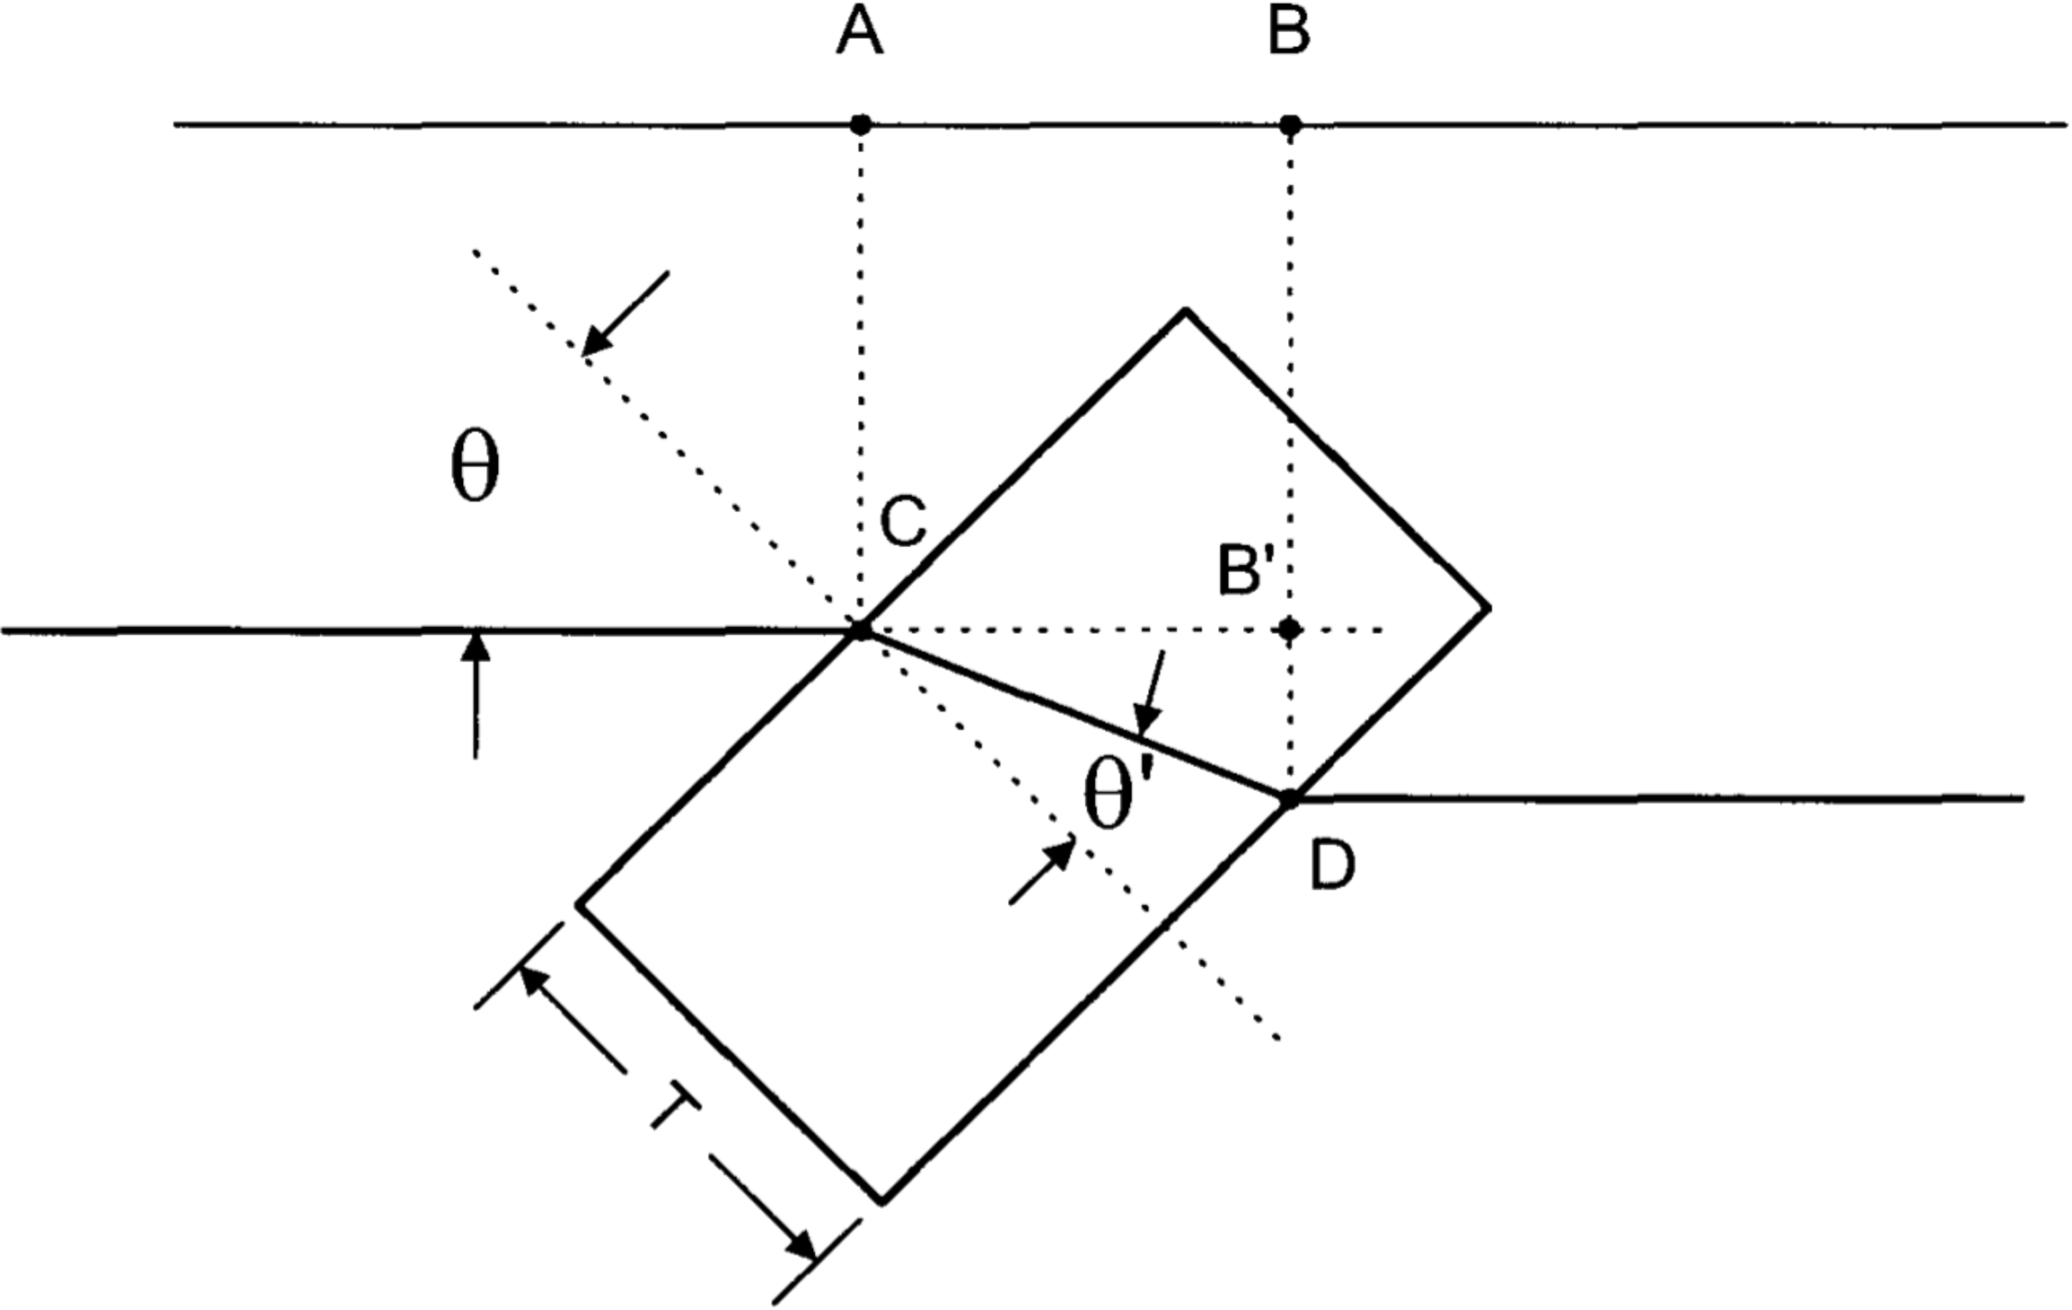
\includegraphics[width=\linewidth]{./figures/glasplaettchen.pdf}
  \caption{The Sagnac Interferometer}
  \label{fig:glasplaettchen}
\end{figure}











% Both beams will have such a phase shift after moving through the distance $L$, and the phase shift will be different since the media are different. But their relative phase shift is just the difference between the total phases. For this reason, the phase shift caused by one beam traveling through a medium of length $L$ while the other travels through a medium with $n \approx 1$ (like the vacuum or air) will be 
% \begin{aquation}
%   \label{eq:phase_shift}
%   \varphi &= \frac{2\pi}{\lambda} (n - 1) L \tp
% \end{aquation}
% The number of interference maxima that occurs due to a phase shift is 
% \begin{aquation}
%   N &= \frac{\varphi}{2\pi} \tp
% \end{aquation}
% Plugging \autoref{eq:phase_shift} into this equation yields 
% \begin{aquation}
%   n &= 1 + \frac{N\lambda}{L} \tc
% \end{aquation}
% which makes it possible to determine the refractive index when $L$, $\lambda$ and $N$ are known.

\subsection{Gaseous Medium}
To measure this index, one of the beam is lead through a gas cell. The difference in the speed of light inside the cell yields a phase difference 
\begin{aquation}
  \Delta \varphi &= \frac{2 \pi L}{\lambda_\text{vac}}\left(n-1\right)
\end{aquation}
between the two beams, which results in them interfering with each other after being reunited. The number of maxima of interference is proportional to the phase difference. It is 
\begin{aquation}
  M &= \frac{\Delta \varphi}{2 \pi} \tp
  \label{eq:interference_maxima}
\end{aquation}
The refractive index is pressure and temperature dependent. To relate it to these quantities, the Lorentz-Lorenz equation 
\begin{aquation}
  \frac{n^2-1}{n^2+1} &= \frac{A p}{R T}
  \label{eq:Lorentz-Lorenz}
\end{aquation}
with pressure $p$, temperature $T$, gas constant $R$ and refractivity $A$.\\
Since the refraction index of air is $\approx 1$, it can be expanded, yielding
\begin{aquation}
  n &= \approx \sqrt{1 + \frac{3 A p}{R T}} \tp
\end{aquation}
This means that the refraction index can be measured by varying the gas's pressure and/or temperature.

% \subsubsection{Solid Medium}
% saf



